\documentclass[conference]{IEEEtran}

\usepackage[utf8]{inputenc}
\usepackage[T1]{fontenc}
\usepackage{graphicx}
\usepackage{textcomp}
\usepackage{breqn}

\title{Application of simple information theory concepts to text analysis and automatic text generation.}
\author{Lorenzo Pistone, 900926-T232, Göteborg University}

\begin{document}

\maketitle

\begin{abstract}
The aim of this paper is to show how simple information theory constructs, such as symbol sequences and correlation information, can be used to analyze texts, and possibly provide a simple algorithm to generate outputs analogous to the sample input text. I will first introduce briefly the quantities involved. Successively, I will explain the algorithm used to store efficiently the conditional probabilities $p(x | \sigma)$ (where $x$ is a symbol and $\sigma$ is the preceding sequence). A text will be analyzed as exemplification. Finally, I will discuss applicability and the limits of this kind of treatment.
\end{abstract}

\IEEEpeerreviewmaketitle

\section{Theoretical introduction}

The first step to analyze a symbol sequence, as a human written text, is to extend the concept of entropy to blocks of data. The fact that a change in the alphabet used to encode a sequence should not change the entropy, leads naturally to the definition of block entropy as

\begin{dmath}
S_m = -\sum_{\sigma_m}p(\sigma_m)\log p(\sigma_m)
\end{dmath}

where $\sigma_m$ is a sequence of symbols of length $m$.

Considering an infinitely long symbol sequence, it is possible to define the entropy per symbol

\begin{dmath}
s = \lim_{m\rightarrow\infty}\frac{S_m}{m}
\end{dmath}

Another way to calculate the entropy per symbol is the mean entropy of the next symbol in the stream, knowing the past sequence and so using the conditional probability $p(x|\sigma_{m-1})$, where $x$ is the new symbol given the past sequence $\sigma$ of length $m-1$:

\begin{dmath}
h_m = \left\langle -\sum_{x}p(x|\sigma_{m-1})\log p(x|\sigma_{m-1})\right\rangle_{\sigma_{m-1}} = -\sum_{\sigma_{m-1}}p(\sigma_{m-1})\sum_{x}p(x|\sigma_{m-1})\log p(x|\sigma_{m-1}) = S_m - S_{m-1} = \Delta S_m
\end{dmath}

Then, by taking the limit $m\rightarrow\infty$, this quantity approaches to $s$. Defining $S_0 = 0$,we get $\Delta S_1 = S_1$.

Finally, let us consider the relative information gained by observing a new symbol after the sequence, an event that changes our probability distribution, because longer correlation lengths can be detected. If we average this quantity over all the possible past sequences of length $m$ we obtain the definition of \emph{correlation information} $k_m$, which, with simple calculations, can be show to equal

\begin{dmath}
k_m = -\Delta S_m + \Delta S_{m-1}
\end{dmath}

$k_1$ is defined as the mean information that we get from changing our probability distribution that describes the stream from a uniform distribution to the actual distribution of single symbols $p(x)$,

\begin{dmath}
k_1 = K[P_1^{uniform}; P_1] = \log \nu - S_1
\end{dmath}

where $\nu$ is the number of symbols in the alphabet. It is easy to show that another expression for the entropy per symbol $s$ is

\begin{dmath}
s = \log \nu - \sum_{m=1}^\infty k_m = \log \nu - k_{corr}
\end{dmath}

where $k_{corr}$ is a measure of the total information located in the correlations.

With these quantities it is possible to measure how much the knowledge of a past symbol sequence can help us in determining what symbol comes next. This can be useful for text generation, but also to develop compression algorithms.

\section{Implementation}

It is evident that all of the quantities described can be built if one knows all the $\Delta S_m$, which in turn requires the calculation of $p(x|\sigma_{m-1})$ and $p(\sigma_{m-1})$.

These probabilities are calculated from the frequency of the tokens found in parsing a sufficiently long input text. Besides obvious computation time limitations, this introduces a first constraint: to have a good statistics, one must input a text much larger than the maximum block of symbols considered, otherwise the probabilities will not be very accurate.

A second problem that is encountered when implementing the algorithm in practice is that if one attempts to store in memory the probability values for all the possible sequences of size $m$, then the used memory goes as $\nu^m$ where $\nu$ is the alphabet size, which becomes prohibitive very quickly if one uses the English alphabet. Yet, it is possible to exploit the fact that a lot of sequences do not appear in the input text, if that is not random but written in a human language.

Following this reasoning, I implemented the structure to record the probabilities as a \emph{trie}. The $p(x)$ is represented as a list of all the possible symbols $x$ for which $p(x)$ is non zero: each element of this list contains the symbol value and the number of occurrences in the text, so that the probability is that number divided by the sum of occurrences of all the possible symbols. Each element of the list contains a link to a list of the successive choices for the next symbol. These latter implicitly assume that the first symbol $x$ has been observed before, so they equal to $p(y|x)$. This can be done recursively to represent $p(z|\sigma)$, where $\sigma$ is a sequence of any length.

If one is interested instead in $p(yx)$, that is the probability of finding $x$ followed by $y$ without knowing that $x$ has just been selected, it is sufficient to normalize the number of occurrences to the total occurrences of all the possible sequences of two symbols. Since we built our probabilities by parsing a text of a certain length, then it is sufficient to divide by $l-1$, where $l$ is the length of the input, because that counts how many two-symbols long sequences we have sampled. Of course, this is easily extended to sequences of length $m$ with $l+1-m$.

This simple scheme allows to save the in memory representation of the big number of newer observed sequences, because it is sufficient not to include a certain symbol in the choice, and the calculation of of the quantities introduced in the previous section is straightforward.

The generation of the new text is performed by choosing a symbol with weights given by $p(x|\sigma)$. It is important to underline the effect of the finiteness of the input text though. It is possible that a certain sequence $\sigma$ of length $m_{MAX}$, the biggest size of the block considered, appears \emph{only} at the end of the inputted text. If the algorithms happens to choose that sequence, after that it will be stuck, because there is no knowledge on what possible sequence could follow. If the length of the input text goes to infinity, this happens with probability that goes to zero. Yet, the algorithm, if such case is detected, will basically start over as if a new text is to be generated after the sequence.

\section{Test case, \emph{The Lord Of The Rings}}

The selected test was \emph{The Lord Of The Rings} by J. R. R. Tolkien. I chose this text because it provides a good long sample, but also because being a narrative book it has some repetitive patterns (like the beginning of speeches).

The algorithm has been run by first translating all the accented vowels to the simple form plu an apostrophe, and newlines have been stripped. The characters included in the alphabet were the English alphabet (distinguishing upper and lower case), white space, and some common punctuation characters (,.;:-?!'). The maximum block length was 51. The plot of $S_m$ follows.

\begin{figure}[h]
\centering
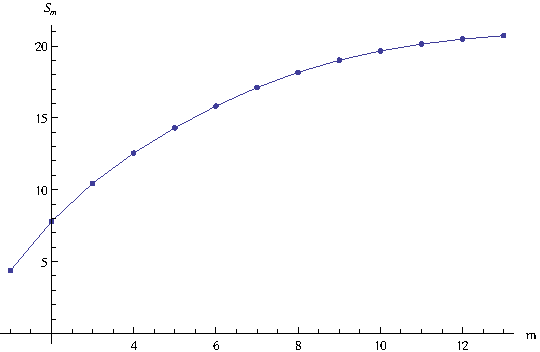
\includegraphics{Sm.pdf}
\caption{$S_m$ for the whole text}
\end{figure}

The block entropy as expected increases as the block length is enlarged. Contrary to the theory, there is a remarkable finite effect. In fact, if one plots all the calculated range of the block size, one gets the following plot.

\begin{figure}[h]
\centering
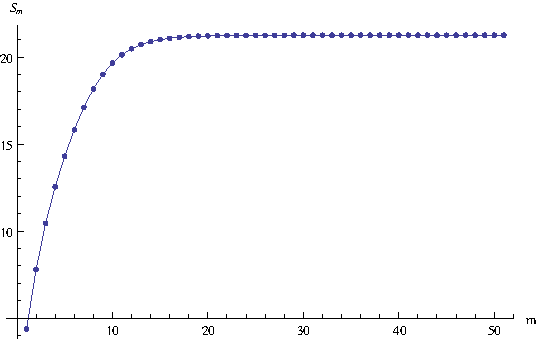
\includegraphics{Sm-extend.pdf}
\caption{$S_m$ for the whole text, extended range}
\end{figure}

After $m \simeq 10$, the block entropy seems to reach a maximum. This leads to a very low entropy per symbol $s$. The explanation is that with blocks of that length, it is very easy for humans to guess what's the next letter, and this is of course the same for the algorithm, hence the next symbol has a very low entropy. This shows the limit of interpreting a human written text is hardly comparable to a stream of symbols, which is one of the assumptions of information theory: this problem will be examined in the next section.

Here follow some lines of generated text for different lengths of allowed ``look-back'' (e.g., $m$ in $p(x|\sigma_m)$), from 1 to 11.

\begin{quote}
1. \emph{t wamsthe d pe th Ho und, t willd tordoum m aneral orre she s th theay. th, avinlabowerolamernd t Sale rbe senithend.}

3. \emph{It change a later about tween deal fling.' 'What downs nowind the mong of the ridge to the Many may own thing a likely prefuge fless. Night. Sam!' 'My don't days therbs of which year up, anyway. Boroming.}

5. \emph{Do you will find it will swords nor ever befell as he cast found before come blindfold, and little his possessed or ignorance the Green', said Frodo forward that has fall of Frodo sat down and ember.}

7. \emph{He was not see how this place.' 'I dare say you not go far.' 'On foot?' cried Pippin. It would not speak more of a hole; but there were set watched the great wolves.}

9. \emph{A great deal from the Shadowy Mountains and laden wains. All people. After they had little faith and high-seat, and then we must go', said Faramir sat down rubbing his speech, and thought secure.}

11. \emph{Darkness came and wings immortal made for him, and without him, and sucked his teeth; and then he remember - if I had seen you before me, if you wish, tell me of this broad hill-back in front.}
\end{quote}

As the block size is increased, grammar is more and more correct. Syntax gets better, but even at big block sizes it is somewhat faulty. Anyway, most of the time the generated sentences do not make sense.

If one selects a very big block, like 25, one does not get anymore a random text, but simply snippet of the input text start being copied. For example one gets

\begin{quote}
25. \emph{The Bree-folk called them Rangers, and knew nothing of their origin. They were taller and darker than the Men of Bree and were believed to have strange powers of sight and hearing, and to understand the languages of beasts and birds.}
\end{quote}

which is a verbatim quote of one of the first chapters. This happens for the same reason for which the entropy does not appear to go to infinity in the extended range graph.

\section{Applicability and limits of the method}

As it is shown in the previous section, this method provides a simple but yet surprisingly good way to generate a random text from a given sample input. It is evident thought that it cannot generate a ``syntactically good'' text. In theory, if one enlarges the maximum size of the sequences considered for the calculation of $p(x|\sigma)$, one can get increasingly better results. Soon though, the big size of the block shrinks the number of different samples that one gets from the inputted text. With big blocks, the algorithm basically starts to copy the input text from a random point, because there are only a few different symbols $x$ for which $p(x|\sigma)$ is different than zero, if $\sigma$ is too large (where ``too large'' depends on the length of the input text).

Increasing the block size is also not sufficient to get an human-like text generator. This can be seen with this simple example. It is common to have sentences in the form ``\emph{if ... then ... else ...}''. To avoid generating sentences that contain one of those three ``keywords'' without a proper structure, one should make sure to have a block size always bigger than the length of any instance of that kind of sentences in the input text. But one can build arbitrarily long ``\emph{if ... then ... else ...}'' sentences, so having a finite maximum size of the considered sequences in the algorithm leads unavoidably to the generation of broken sentences. It is evident then that a less naive attempt to generate texts cannot just rely on correlations over a fixed block length. Some tools, like context-free grammars, allow a more high level and efficient algorithms, but they usually require the explicit description of the grammar rules: for this reason they have nothing to do with information theory, whose approach is to treat the data just as a stream of symbols, hence these methods are out of the scope of this document.

\end{document}
